\documentclass[../main]{subfiles}
\begin{document}

\chapter{展示}%
\label{cha:display}

\begin{figure}[htbp]
  \centering
  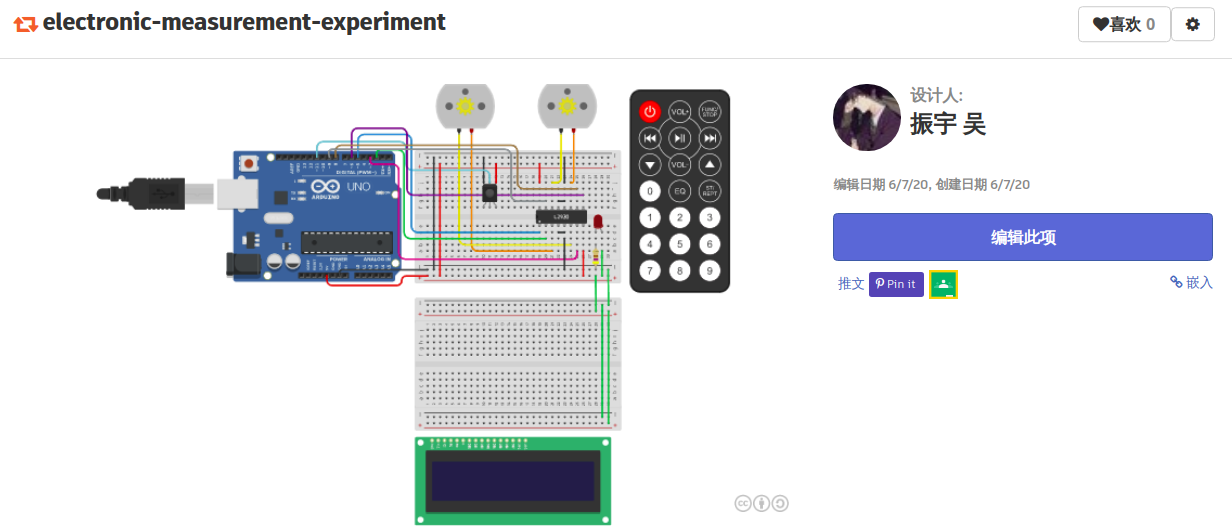
\includegraphics[
    width = \linewidth,
  ]{simulate}
  \caption{仿真}%
  \label{fig:simulate}
\end{figure}

\begin{figure}[htbp]
  \centering
  \begin{subfigure}[htbp]{0.8\linewidth}
    \centering
    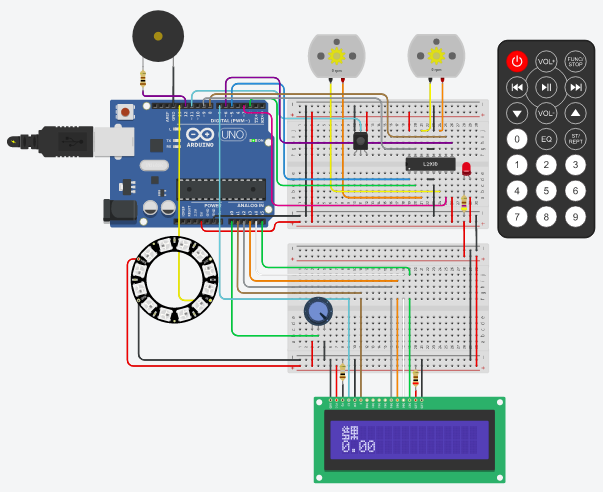
\includegraphics[
    width = \linewidth,
    ]{display/0}
    \caption{模拟信号最小}%
    \label{fig:display/0}
  \end{subfigure}
  \quad
  \begin{subfigure}[htbp]{0.8\linewidth}
    \centering
    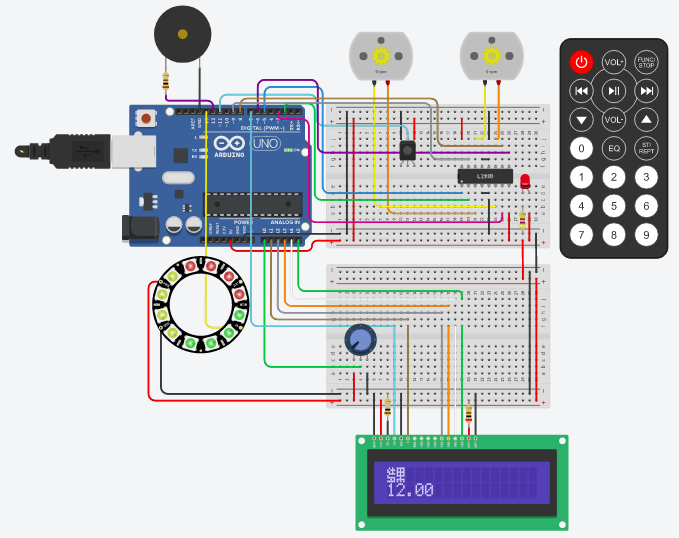
\includegraphics[
    width = \linewidth,
    ]{display/12}
    \caption{模拟信号最大}%
    \label{fig:display/12}
  \end{subfigure}
  \caption{展示}%
  \label{fig:display}
\end{figure}

\end{document}

